\section{Applications}

\subsection{Overview}

Traditional applications can not achieve complicated and efficient goals due 
to the limited processing power and memory space of sensors.

In our system, applications for wireless sensor networks are inspired by 
greater potential with the UAV based SDN controller. The central controller
helps sensors execute complex calculations such as AI model training, as well 
as store global information. Besides, UAVs have flexible features and can deploy 
tasks to sensors by one-hop communication directly. Thus it enables the sensor network
to achieve much more intelligent applications.

In our system, applications can be found for a variety of purposes, including routing, AI node selection,
Ai energy prediction, multi-tasks and network diagnosis. We design all these applications and provide 
easy-to-use interfaces to users as in Table \ref{API}.



\subsection{Routing}

\subsection{AI Node Selection}

\subsubsection{Motivation}

\subsubsection{Design}

Greedy selection algorithm.

\begin{algorithm}
\caption{Greedy Selection Algorithm}
\label{Greedy}
\begin{algorithmic}[1]
\STATE Input: Sensor set $N$, Selected set $M$, Target area $\Omega$, Covering area $\Phi$;
\STATE Initialize : $N = \emptyset$, $\Phi = \emptyset$
\WHILE {$M \neq N$}
    \IF{$\Phi = \Omega $}
        \STATE break; $\backslash$$\backslash$ selected set has been found
    \ENDIF
    \STATE Find $n_i : argmax(\Phi \cap range(n))$, $n_i \in (N-M)$;
    \STATE $\Phi = \Phi \cup {n_i}$
\ENDWHILE
\end{algorithmic}
\end{algorithm}

SRSSS AI algorithm selection.

\begin{figure}[htbp]
	\centering
	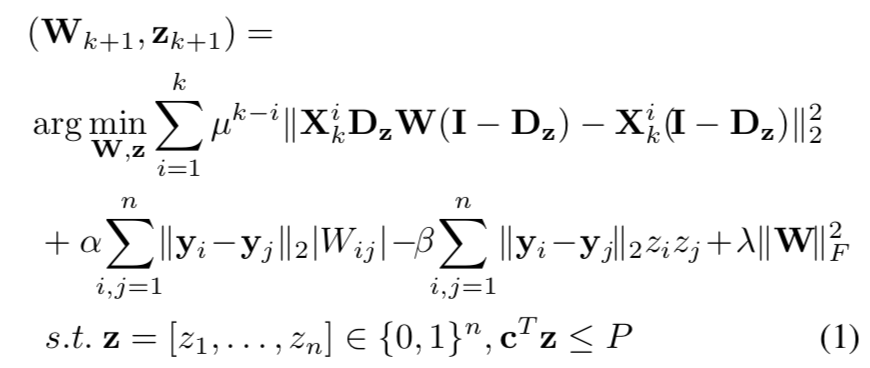
\includegraphics[width=2in]{Figure/OF}
	\caption{Objective function.}
	\label{system}
\end{figure}


**************

AI helps creating smarter sensor systems.

AI systems have been improving, and new advances in machine intelligence are creating seamless interactions between people and digital sensor systems.

 In sensor systems, applications can be found for a variety of tasks, including selection of sensor inputs, interpreting signals, condition monitoring, fault diagnosis, machine and process control, machine design, process planning, production scheduling, and system configuring. Some examples of specific tasks undertaken by expert systems are:
* Assembly 
* Automatic programming 
* Controlling intelligent complex vehicles  
* Planning inspection 
* Predicting risk of disease 
* Selecting tools and machining strategies 
* Sequence planning 
* Controlling plant growth. 

AI can increase effective communication, reduce mistakes, minimize errors, and extend sensor life.



The tools and methods described have minimal computation complexity and can be implemented on small assembly lines, single robots, or systems with low-capability microcontrollers. These novel approaches proposed use ambient intelligence and the mixing of different AI tools in an effort to use the best of each technology. The concepts are generically applicable across many processes.


minimum energy, data loss, reliability, robustness, etc., in place during the design and operation of wireless sensor networks

a specific set of protocols for medium access, localization and positioning, time synchronization, topology control, security and routing are identified based on the current configuration of the network, the requirements of the application and the topology of their deployment.

\subsection{AI Energy Prediction}

\subsubsection{Motivation}

\subsubsection{Design}

\subsection{Multi-tasks}

\subsubsection{Motivation}

A software defined sensor node can perform multiple tasks.

wireless sensor network(WSN) are generally comprised of a group of 
spatially dispersed sensors, monitoring and recording the physical conditions
of the environment. WSNs measure environmental conditions like temperature, sound, sunlight,
humidity, etc.

A deployed wireless sensor networks are usually assigned  

In our system, a sensor node can perform multiple tasks with different sensing targets simultaneously.

A sensor node may have different sensing ranges for different tasks.

only the sensor node loaded with a program for task can sense targets.

There are several practical requirements.

Different tasks have different requirements, including time, sensing range, sensing ratio, etc.

For example tasks like sunlight collection only need to be carried out during the daytime.

Our system provide a task scheduling to 

Sensors are usually assigned multi-tasks.

\subsubsection{Design}

Sensors are assigned tasks to monitor a specific area.

Different tasks have different requirements, including time, density, etc.

Task scheduler do the arrangement. 

Task buffer.

Task queue.

Scheduling table.

...

\subsection{Network Diagnosis}

Diagnose the network.
